\documentclass[a4paper]{scrartcl}

\usepackage[
	fancytheorems, 
	fancyproofs, 
	noindent
]{adam}

\usepackage{cancel}
\usepackage{tikz}

% \allowdisplaybreaks

\title{Probability}
\author{Adam Kelly (\texttt{ak2316@cam.ac.uk})}
\date{\today}

\begin{document}

\maketitle


This handout is a crash course which covers the basic ideas of an introductory and not \emph{completely} (but mostly) rigorous probability course. 
Many, many details will \emph{not} be spelled out (though we won't write anything incorrect), and some `mathematical extrapolation' will be needed to derive any significant value from this handout. You have been warned -- have fun!

\tableofcontents

\section{Setting Up Probability}

We are going to build up probability from the very basic axioms. This will give us a firm mathematical basis to work from, but also will match the intuitive notions of probability that you have hopefully developed before reading this handout.

\subsection{Probability Spaces}

The basic object of study in probability theory is that of \emph{probability spaces}. We begin by defining how we can talk about the idea of `events' formally. What we want from our definition will be some way to have a set of possible `outcomes' (a \emph{sample space}), from which we can combine different outcomes to form various `events'. This leads almost directly to the definition of an \emph{event space}.

\begin{definition}[Event Space] The collection $\FF$ of subsets of the sample space $\Omega$ is an \vocab{event space} or \vocab{$\sigma$-algebra} if
	\begin{enumerate}
		\item $\FF$ is non-empty,
		\item if $A \in \FF$, then $\Omega \backslash A \in \FF$,
		\item if $A_1, A_2, \dots \in \FF$, then $\bigcup_{i = 1}^{\infty} A_i \in \FF$.
	\end{enumerate}
\end{definition}

Within this system, $A \cup B$ corresponds to either $A$ or $B$ occurring, $A \cap B$ corresponds to both $A$ and $B$ occurring, and $\Omega \backslash A$ corresponds with anything but $A$ occurring. You get the idea.

Our main goal in the study of probability is to assign some sort of `likelihood' to events in the event space. This is done through the introduction of a \emph{probability measure}.


\begin{definition}[Probability Measure]
	We say that a function $\PP : \FF \rightarrow \R$ is a \vocab{probability measure} on $(\Omega, \FF)$ if
	\begin{enumerate}
		\item $\PP(A) \geq 0$ for all $A \in \FF$,
		\item $\PP(\Omega) = 1$,
		\item if $A_1, A_2, \dots$ are disjoint events in $\FF$, then $\PP\left(\bigcup_{i = 1}^{\infty} A_i\right) = \sum_{i = 1}^{\infty} \PP(A_i)$.
	\end{enumerate} 
\end{definition}

These properties of the probability measure should match your own intuition about the way that probability works. Putting all the pieces together, we get our main object of study: the \emph{probability space}.

\begin{definition}[Probability Space]
	A \vocab{probability space} is a triple $(\Omega, \FF, \PP)$ such that $\Omega$ is non empty, $\FF$ is an event space on $\Omega$, and $\PP$ is a probability measure on $(\Omega, \FF)$.
\end{definition}


If we only have to deal with say finite (or even countable) $\Omega$, then it makes sense to usually take $\FF$ to just be the power set of $\Omega$. In this case, if $\Omega = \{\omega_1, \omega_2, \dots \}$, then we can construct any probability measure $\PP$ by just specifying $\PP(\{\omega_i\})$ for all $i$, as then for $A \in \FF$, we can get $\PP(A) = \sum_{\omega \in A} \PP(\{\omega\})$. 

\subsection{Conditional Probability and Independence}

In our day-to-day experience, we know that knowledge about one event can influence how likely we determine another event is to occur. This type of thinking motivates the introduction of \emph{conditional probability}.

\begin{definition}[Conditional Probability]
	If $A, B \in \FF$ and $\PP(B) > 0$, the \vocab{probability of $A$ given $B$} is denoted $\PP(A \mid B)$, and is given by
	$$
	\PP(A \mid B) = \frac{\PP(A \cap B)}{\PP(B)}.
	$$
\end{definition}

It's not hard to check that $\PP(\; \cdot \mid B)$ is a probability measure, as we would expect -- it's just assigning probabilities to events in $\FF$ in a different way!

A natural thing to care about is if knowledge about an event \emph{doesn't} influence how likely another event is. We call such events independent.

\begin{definition}[Independent Events]
We say that events $A, B$ in a probability space $(\Omega, \FF, \PP)$ are \vocab{independent} if
$$
\PP(A \cap B) = \PP(A) \PP(B),
$$
and \vocab{dependent} otherwise.
\end{definition}

We can see immediately that $A, B$ independent implies that
$$
\PP(A \mid B) = \PP(A) \quad \text{and} \quad \PP(B \mid A) = \PP(B),
$$
if $\PP(A), \PP(B) \neq 0$. However, this definition is slightly more general than this property since it handles events with zero probability.
We can generalise this notion of independence to multiple events, and we get a criterion that's stronger than pairwise independence\footnote{It's not hard to construct an example of events that are pairwise independent but wouldn't be independent in any reasonable sense.}.

\begin{definition}[Mutually Independent Events]
	We say that the events $A_1$, $A_2$, $A_3$, $\dots$ are \vocab{mutually independent} if
	$$
	\PP(A_{i_1} \cap A_{i_2} \cap \cdots \cap A_{i_r}) = \PP(A_{i_1}) \PP(A_{i_2}) \cdots \PP(A_{i_r}),
	$$
	for any $i_1, i_2, \dots, i_r$ and $r \geq 2$.
\end{definition}

So if conditional probability tells us about the likelihood of a certain event in one particular scenario, then it's easy to imagine that knowing about the likelihood in every scenario would then just give you the likelihood in general. Such thinking is formalised in the \emph{law of total probability}, also known as the \emph{partition theorem}.

\begin{theorem}[Partition Theorem]
	Let $\{B_1, B_2, \dots\}$ be a collection of disjoint events such that $\PP(B_i) > 0$ for all $i$ and $\bigcup_{i = 1}^{\infty} B_i = \Omega$. Then
	$$
	\PP(A) = \sum_i \PP(A \mid B_i) \PP(B_i),
	$$
	for any $A \in \FF$.
\end{theorem}
\begin{proof}
	We can compute that
	\begin{align*}
		\sum_{i} \PP(A \mid B_i) \PP(B_i) &= \sum_i \PP(A \cap B_i) = \PP\left(\bigcup_i (A \cap B_i)\right) = \PP(A),
	\end{align*}
	as required.
\end{proof}

Using the partition theorem, we can establish the famous \vocab{Bayes' theorem}, which allows us to use knowledge about $\PP(A \mid B_j)$ to give information about $\PP(B_j \mid A)$:
$$
\PP(B_j \mid A) = \frac{\PP(A \mid B_j) \PP(B_j)}{\PP(A)} = \frac{\PP(A \mid B_j) \PP(B_j)}{\sum_i \PP(A \mid B_i) \PP(B_i)}.
$$



\subsection{Continuity of Probability Measures}

In the definitions for event spaces ($\sigma$-algebras) and probability measures, you may notice that we specify rules for countably infinite sequences of events. This is for good reason -- there's plenty of natural scenarios where such a setup is useful. For example, consider the experiment of tossing a coin until you get heads, in which it is possible to get an arbitrarily long run of tails before you stop tossing. To make working with such scenarios easier, we can establish a result which allows us study events as limits of a sequence of events -- that the probability measure is continuous.


\begin{definition}[Limits of Events]
	We say that a sequence of events $A_1, A_2, \dots$ is \emph{increasing} if $A_1 \subseteq A_2 \subseteq \cdots$. We define the \vocab{limit} as
	$$
	\lim_{n \to \infty} A_n = \bigcup_{n = 1}^{\infty} A_n.
	$$
\end{definition}

\begin{theorem}[Continuity of Probability Measures]
	Let $(\Omega, \FF,\PP)$ be a probability space. If $A_1, A_2, \dots$ is an increasing sequence of events in $\FF$ with limit $A$, then $\PP(A) = \lim_{n \to \infty} \PP(A_n)$.
\end{theorem}
\begin{proof}
	Define $B_i = A_i \backslash A_{i - 1}$, with $B_1 = A_1$. Then we have
	$$
A = B_1 \cup B_2 \cup B_3 \cup \cdots
	$$
	which is the union of disjoint events in $\FF$. Thus we have
	\begin{align*}
		\PP(A) &= \PP\left(\bigcup_{n = 1}^{\infty} A_n\right) = \PP\left(\bigcup_{n = 1}^{\infty} B_n\right) \\
		&= \lim_{n \to \infty} \sum_{i = 1}^{n} \PP(B_n) = \lim_{n \to \infty} \PP(B_1 \cup \cdots \cup B_n) \\ &= \lim_{n \to \infty} \PP(A_n),
	\end{align*}
	as required.
\end{proof}

As a side note, the type of construction used to define $B_i$ can be quite helpful when we want to deal with a disjoint union, rather than some non-disjoint sequence of events (since it works nicely with the definition of the probability space!)

% Another rather intuitive notion is that or probabilities being `subadditive' when events are \emph{not} disjoint, which we can see in the following result.

% \begin{theorem}[Boole's Inequality -- The Union Bound]
% 	For any sequence of events $A_1, A_2, \dots$ we have
% 	$$
% 	\PP\left(\bigcup_{i = 1}^{\infty} A_i\right) \leq \sum_{i = 1}^{\infty} \PP(A_i).
% 	$$
% \end{theorem}
% \begin{proof}
% 	We use a similar construction to the previous proof. Let $B_1 = A_1$, and define $B_i = A_i \backslash \bigcup_{k = 1}^{i - 1} A_k$. Then we have
% 	$$
% 	\PP\left(\bigcup_{i = 1}^{\infty} A_i\right) = \PP\left(\bigcup_{i = 1}^{\infty} B_i\right) = \sum_{i = 1}^{\infty} \PP(B_i) \leq \sum_{i = 1}^{\infty} \PP(A_i),
% 	$$
% 	where inequality occurs since $\PP(A_i) = \PP(B_i) + \PP\left(\bigcup_{k = 1}^{i - 1} A_i\right) \geq \PP(B_i)$.
% \end{proof}


\section{Discrete Random Variables}

Imagine the following scenario. You are in a lecture hall, and you decide to perform an experiment where choose a student at random and ask them how they performed in the admissions test. It would be natural to model this scenario with a probability space $(\Omega, \FF, \PP)$ where $\Omega = \{\omega_1, \dots, \omega_n\}$ where each $\omega_i$ corresponds to a student in the lecture hall, $\FF$ is all possible subsets of $\Omega$, and $\PP$ is the probability measure describing the likelihoods of given students being chosen in the experiment.

So how does the `asking for the student's test score' fit into this setup? A natural way to deal with this is by defining a function $X : \Omega \rightarrow \R$ where $X(\omega_i)$ is the admissions test score of the student $\omega_i$. We call such a function a \emph{discrete random variable}. 

\begin{definition}[Discrete Random Variables]
	A \vocab{discrete random variable} $X$ on a probability space $(\Omega, \FF, \PP)$ is a function $X : \Omega \rightarrow \R$ such that the image $X(\Omega)$ is a countable subset of $\R$ and $\{ \omega \in \Omega : X(\omega) = x \} \in \FF$ for $x \in \R$.
\end{definition}

A natural mental picture to go along with this definition (which roughly follows our motivating example) is shown below.

\begin{center}
	

\tikzset{every picture/.style={line width=0.75pt}} %set default line width to 0.75pt        

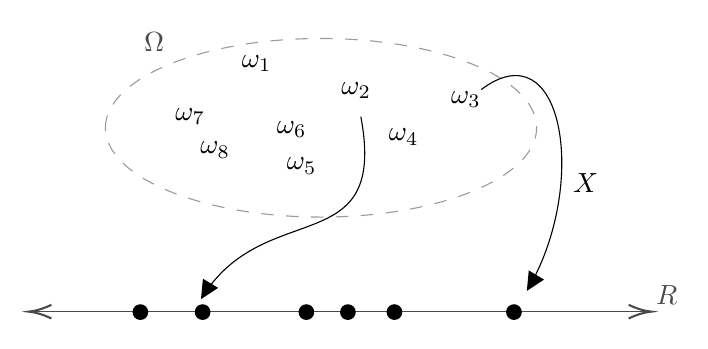
\begin{tikzpicture}[x=0.75pt,y=0.75pt,yscale=-1,xscale=1]
%uncomment if require: \path (0,300); %set diagram left start at 0, and has height of 300

%Shape: Ellipse [id:dp9108797218897698] 
\draw  [color={rgb, 255:red, 155; green, 155; blue, 155 }  ,draw opacity=1 ][dash pattern={on 4.5pt off 4.5pt}] (56.95,71.41) .. controls (56.95,47.65) and (103.46,28.39) .. (160.83,28.39) .. controls (218.21,28.39) and (264.71,47.65) .. (264.71,71.41) .. controls (264.71,95.17) and (218.21,114.43) .. (160.83,114.43) .. controls (103.46,114.43) and (56.95,95.17) .. (56.95,71.41) -- cycle ;
%Straight Lines [id:da6842961904360465] 
\draw [color={rgb, 255:red, 74; green, 74; blue, 74 }  ,draw opacity=1 ]   (22,160) -- (318,160) ;
\draw [shift={(320,160)}, rotate = 180] [color={rgb, 255:red, 74; green, 74; blue, 74 }  ,draw opacity=1 ][line width=0.75]    (10.93,-3.29) .. controls (6.95,-1.4) and (3.31,-0.3) .. (0,0) .. controls (3.31,0.3) and (6.95,1.4) .. (10.93,3.29)   ;
\draw [shift={(20,160)}, rotate = 0] [color={rgb, 255:red, 74; green, 74; blue, 74 }  ,draw opacity=1 ][line width=0.75]    (10.93,-3.29) .. controls (6.95,-1.4) and (3.31,-0.3) .. (0,0) .. controls (3.31,0.3) and (6.95,1.4) .. (10.93,3.29)   ;
%Shape: Circle [id:dp7950112027979597] 
\draw  [draw opacity=0][fill={rgb, 255:red, 0; green, 0; blue, 0 }  ,fill opacity=1 ] (100,160.21) .. controls (100,158.12) and (101.69,156.43) .. (103.79,156.43) .. controls (105.88,156.43) and (107.57,158.12) .. (107.57,160.21) .. controls (107.57,162.31) and (105.88,164) .. (103.79,164) .. controls (101.69,164) and (100,162.31) .. (100,160.21) -- cycle ;
%Shape: Circle [id:dp6131304198024731] 
\draw  [draw opacity=0][fill={rgb, 255:red, 0; green, 0; blue, 0 }  ,fill opacity=1 ] (170,160.21) .. controls (170,158.12) and (171.69,156.43) .. (173.79,156.43) .. controls (175.88,156.43) and (177.57,158.12) .. (177.57,160.21) .. controls (177.57,162.31) and (175.88,164) .. (173.79,164) .. controls (171.69,164) and (170,162.31) .. (170,160.21) -- cycle ;
%Shape: Circle [id:dp9238073836570526] 
\draw  [draw opacity=0][fill={rgb, 255:red, 0; green, 0; blue, 0 }  ,fill opacity=1 ] (192.43,160.21) .. controls (192.43,158.12) and (194.12,156.43) .. (196.21,156.43) .. controls (198.31,156.43) and (200,158.12) .. (200,160.21) .. controls (200,162.31) and (198.31,164) .. (196.21,164) .. controls (194.12,164) and (192.43,162.31) .. (192.43,160.21) -- cycle ;
%Shape: Circle [id:dp2974634348831592] 
\draw  [draw opacity=0][fill={rgb, 255:red, 0; green, 0; blue, 0 }  ,fill opacity=1 ] (250,160.21) .. controls (250,158.12) and (251.69,156.43) .. (253.79,156.43) .. controls (255.88,156.43) and (257.57,158.12) .. (257.57,160.21) .. controls (257.57,162.31) and (255.88,164) .. (253.79,164) .. controls (251.69,164) and (250,162.31) .. (250,160.21) -- cycle ;
%Shape: Circle [id:dp34244152371437553] 
\draw  [draw opacity=0][fill={rgb, 255:red, 0; green, 0; blue, 0 }  ,fill opacity=1 ] (70,160.21) .. controls (70,158.12) and (71.69,156.43) .. (73.79,156.43) .. controls (75.88,156.43) and (77.57,158.12) .. (77.57,160.21) .. controls (77.57,162.31) and (75.88,164) .. (73.79,164) .. controls (71.69,164) and (70,162.31) .. (70,160.21) -- cycle ;
%Shape: Circle [id:dp8457167113190215] 
\draw  [draw opacity=0][fill={rgb, 255:red, 0; green, 0; blue, 0 }  ,fill opacity=1 ] (150,160.21) .. controls (150,158.12) and (151.69,156.43) .. (153.79,156.43) .. controls (155.88,156.43) and (157.57,158.12) .. (157.57,160.21) .. controls (157.57,162.31) and (155.88,164) .. (153.79,164) .. controls (151.69,164) and (150,162.31) .. (150,160.21) -- cycle ;
%Curve Lines [id:da9264222857198537] 
\draw    (238,53) .. controls (277.4,23.45) and (289.77,97.58) .. (261.33,147.73) ;
\draw [shift={(260,150)}, rotate = 301.01] [fill={rgb, 255:red, 0; green, 0; blue, 0 }  ][line width=0.08]  [draw opacity=0] (8.93,-4.29) -- (0,0) -- (8.93,4.29) -- cycle    ;
%Curve Lines [id:da22175284361216296] 
\draw    (180,66) .. controls (193.09,135.65) and (134.93,104.82) .. (104.38,151.8) ;
\draw [shift={(103,154)}, rotate = 301.01] [fill={rgb, 255:red, 0; green, 0; blue, 0 }  ][line width=0.08]  [draw opacity=0] (8.93,-4.29) -- (0,0) -- (8.93,4.29) -- cycle    ;

% Text Node
\draw (89.43,60.87) node [anchor=north west][inner sep=0.75pt]    {$\omega _{7}$};
% Text Node
\draw (138.29,67.29) node [anchor=north west][inner sep=0.75pt]    {$\omega _{6}$};
% Text Node
\draw (101.43,77.01) node [anchor=north west][inner sep=0.75pt]    {$\omega _{8}$};
% Text Node
\draw (143.14,84.71) node [anchor=north west][inner sep=0.75pt]    {$\omega _{5}$};
% Text Node
\draw (169.43,48.4) node [anchor=north west][inner sep=0.75pt]    {$\omega _{2}$};
% Text Node
\draw (192.29,70.77) node [anchor=north west][inner sep=0.75pt]    {$\omega _{4}$};
% Text Node
\draw (121.43,35.38) node [anchor=north west][inner sep=0.75pt]    {$\omega _{1}$};
% Text Node
\draw (222.29,52.8) node [anchor=north west][inner sep=0.75pt]    {$\omega _{3}$};
% Text Node
\draw (74.29,24.28) node [anchor=north west][inner sep=0.75pt]  [color={rgb, 255:red, 74; green, 74; blue, 74 }  ,opacity=1 ]  {$\Omega $};
% Text Node
\draw (321,158) node [anchor=south west] [inner sep=0.75pt]  [color={rgb, 255:red, 74; green, 74; blue, 74 }  ,opacity=1 ]  {$\mathbb{R}$};
% Text Node
\draw (281,92) node [anchor=north west][inner sep=0.75pt]    {$X$};


\end{tikzpicture}

\end{center}

% \clearpage

\subsection{Probability Mass Functions}

With the introduction of discrete random variables, we can change our view from probabilities of events occurring to the probabilities that a discrete random variable takes on specific values. A nice way to do this is by introducing the \emph{probability mass function}.

\begin{definition}[Probability Mass Function]
	The \vocab{probability mass function} or \vocab{pmf} of a discrete random variable $X$ is a function $p_X: \R \rightarrow [0, 1]$ defined by
	$$
	p_X(x) = \PP(X = x) = \PP(\{ \omega \in \Omega : X(\omega) = x\}).
	$$
\end{definition}

It turns out that the probability mass function encodes pretty much all information about the discrete random variable $X$, so much so that if we have some function $p_X$ that acts like a probability mass function, we can say things like `let $X$ be a random variable taking value $x_i$ with probability $p_X(x_i)$' and have it be completely well defined.

\begin{theorem}
	Let $p_X : \R \rightarrow [0, 1]$ be a function such that $p_X(x) \neq 0$ for countably many $x$ and $\sum_{x \in \R} p_X(x) = 1$. Then there is a probability space $(\Omega, \FF, \PP)$ and a random variable $X$ on this space where $X$ has probability mass function $p_X$.
\end{theorem}
\begin{proof}
	Take $\Omega = \{x \in \R : p_X(x) \neq 0\}$, $\FF$ to be all subsets of $\Omega$, and 
	$$
	\PP(A) = \sum_{\omega \in A} p_X(\omega) \quad \text{for }A \in \FF,
	$$
	and define $X : \Omega \rightarrow \R$ by $X(\omega) = \omega$.
\end{proof}


\subsection{Expected Value}

A common question when dealing with discrete random variables is `what is the mean of this discrete random variable?'. Thinking back to our 
lecture hall example, this would correspond with asking what the mean test score in the lecture hall was.
We answer such questions by defining the \emph{expectation} of a random variable.

\begin{definition}[Expected Value]
	If $X$ is a discrete random variable, we define the \vocab{expected value} of $X$ to be
	$$
\EE[X] = \sum_{x \in \img X} x \PP(X = x)
	$$
	whenever this sum converges absolutely\footnote{We require this because we rearranging the sum shouldn't change the expected value -- see Analysis I.}.
\end{definition}

There are a few `tricks' which make the computation of expected value somewhat easier. For example, if we have a discrete random variable defined on some probability space $(\Omega, \FF, \PP)$, then we can sum over the elements of $\Omega$ rather than the elements of $\img X$.
Also, since random variables are really just functions, we can obtain new random variables by composing them with other functions, for example $X \mapsto X^2$. In such scenarios, we can use a seemingly obvious result.

\begin{theorem}[Law of The Subconscious Statistician]
	If $X$ is a discrete random variable and $g: \R \rightarrow \R$, then
	$$
\EE[g(X)] = \sum_{x \in \img X} g(x) \PP(X = x),
	$$
	whenever this sum converges absolutely.
\end{theorem}
\begin{proof}
	Let $Y = g(X)$ be a discrete random variable. Then
	\begin{align*}
		\EE[Y] &= \sum_{y \in \img Y} y \PP(Y = y) = \sum_{y \in \img Y} y \sum_{x \in \img X : g(x) = y} \PP(X = x)  \\
		&= \sum_{x \in \img X} g(x) \PP(X = x),
	\end{align*}
	provided this converges absolutely.
\end{proof}

Another thing we can do very easily is find the expected value of a sum of random variables, using \emph{linearity of expectation}.

\begin{theorem}[Linearity of Expectation]
	For any random variables $X_1, X_2, \dots, X_n$ for which the following expectations exist,
	$$
\EE\left[X_1 + \cdots + X_n\right]= \EE[X_1] + \cdots + \EE[X_n].
	$$
\end{theorem}
\begin{proof}
	We sum over the elements of the sample space $\Omega$ to get
	\begin{align*}
		\EE[X] &= \sum_{\omega \in \Omega} p(\omega)[X_1(\omega) + \cdots + X_n(\omega)]\\
		&= \sum_{\omega \in \Omega} p(\omega) X_1(\omega) + \cdots + \sum_{\omega \in \Omega} p(\omega) X_n(\omega)\\&= \EE[X_1] + \cdots + \EE[X_n].
	\end{align*}
\end{proof}

It's important to note that there's absolutely no requirement that the random variables be independent for this to hold -- one of the reasons why it's an incredibly useful result!

So if expected value measures something like the `mean' of a random variable, it's natural to think about how we can measure how we can expect the random variable deviates from this mean. This is done through the notion of \emph{variance}.

\begin{definition}[Variance]
	The \vocab{variance} $\var(X)$ of a discrete random variable $X$ is defined to be
	$$
\var(X) = \EE[(X - \EE[X])^2].
	$$
\end{definition}

By just working through the definitions we can see that $\var(X) = \EE[X^2] - \EE[X]^2$, which is often an easy way to calculate this quantity.

\subsection{Indicator Functions}

There's one type of random variable which is so useful that it needs to be brought to your attention immediately -- indicator functions.

\begin{definition}[Indicator Functions]
	The \vocab{indicator function} of an event $A$ is the random variable $\ii_A$ where
	$$
\ii_A(\omega) = \begin{cases}
	1 &\mbox{if } \omega  \in A, \\
	0 &\mbox{if } \omega  \not \in A.
   \end{cases}
	$$
\end{definition}

Indicator functions have nice algebraic facts which reflect common ways to manipulate events:
\begin{align*}
	\ii_{A^c} &= 1 - \ii_A, \\
	\ii_{A \cap B} &= \ii_A \ii_B, \\
	\ii_{A \cup B} &= \ii_A + \ii_B - \ii_A \ii_B.
\end{align*}
Still one of the best things about indicator functions is that they allow us to talk about probabilities of events using expectations, since
$$
\EE[\ii_A]= \PP(A).
$$
All of these properties are straightforward and easy to check (just do casework), but they can make proving things and solving problems much easier. Nontrivial example time!

\begin{example}[Solving Problems With Indicator Functions]
A total of $n$ bar magnets are placed end to end in a line with random independent orientations. Adjacent like poles repel, ends with opposite polarities join to form blocks. Let $X$ be the number of blocks of joined magnets. Find $\mathbb{E}[X]$ and $\var(X)$.
\end{example}
\begin{proof}[Solution]
	The situation looks something like this:
	\begin{center}
		

\tikzset{every picture/.style={line width=0.75pt}} %set default line width to 0.75pt        

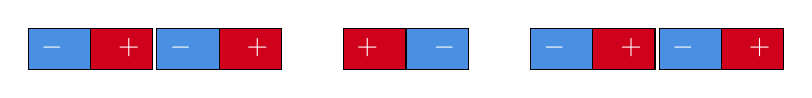
\begin{tikzpicture}[x=0.75pt,y=0.75pt,yscale=-1,xscale=1]
%uncomment if require: \path (0,300); %set diagram left start at 0, and has height of 300

%Shape: Rectangle [id:dp25601061256284363] 
\draw  [fill={rgb, 255:red, 74; green, 144; blue, 226 }  ,fill opacity=1 ] (78,230) -- (108,230) -- (108,250) -- (78,250) -- cycle ;
%Shape: Rectangle [id:dp6474954982899106] 
\draw  [fill={rgb, 255:red, 208; green, 2; blue, 27 }  ,fill opacity=1 ] (108,230) -- (138,230) -- (138,250) -- (108,250) -- cycle ;
%Shape: Rectangle [id:dp4965245878027762] 
\draw  [fill={rgb, 255:red, 74; green, 144; blue, 226 }  ,fill opacity=1 ] (140,230) -- (170,230) -- (170,250) -- (140,250) -- cycle ;
%Shape: Rectangle [id:dp1858582011582739] 
\draw  [fill={rgb, 255:red, 208; green, 2; blue, 27 }  ,fill opacity=1 ] (170,230) -- (200,230) -- (200,250) -- (170,250) -- cycle ;
%Shape: Rectangle [id:dp8867339379180033] 
\draw  [fill={rgb, 255:red, 208; green, 2; blue, 27 }  ,fill opacity=1 ] (230,230) -- (260,230) -- (260,250) -- (230,250) -- cycle ;
%Shape: Rectangle [id:dp33998768810132374] 
\draw  [fill={rgb, 255:red, 74; green, 144; blue, 226 }  ,fill opacity=1 ] (260,230) -- (290,230) -- (290,250) -- (260,250) -- cycle ;
%Shape: Rectangle [id:dp09533432318082213] 
\draw  [fill={rgb, 255:red, 74; green, 144; blue, 226 }  ,fill opacity=1 ] (320,230) -- (350,230) -- (350,250) -- (320,250) -- cycle ;
%Shape: Rectangle [id:dp9775009294983759] 
\draw  [fill={rgb, 255:red, 208; green, 2; blue, 27 }  ,fill opacity=1 ] (350,230) -- (380,230) -- (380,250) -- (350,250) -- cycle ;
%Shape: Rectangle [id:dp24270866646840328] 
\draw  [fill={rgb, 255:red, 74; green, 144; blue, 226 }  ,fill opacity=1 ] (382,230) -- (412,230) -- (412,250) -- (382,250) -- cycle ;
%Shape: Rectangle [id:dp11919818567548779] 
\draw  [fill={rgb, 255:red, 208; green, 2; blue, 27 }  ,fill opacity=1 ] (412,230) -- (442,230) -- (442,250) -- (412,250) -- cycle ;

% Text Node
\draw (120,233.4) node [anchor=north west][inner sep=0.75pt]  [color={rgb, 255:red, 255; green, 255; blue, 255 }  ,opacity=1 ]  {$+$};
% Text Node
\draw (83,233.4) node [anchor=north west][inner sep=0.75pt]  [color={rgb, 255:red, 255; green, 255; blue, 255 }  ,opacity=1 ]  {$-$};
% Text Node
\draw (182,233.4) node [anchor=north west][inner sep=0.75pt]  [color={rgb, 255:red, 255; green, 255; blue, 255 }  ,opacity=1 ]  {$+$};
% Text Node
\draw (145,233.4) node [anchor=north west][inner sep=0.75pt]  [color={rgb, 255:red, 255; green, 255; blue, 255 }  ,opacity=1 ]  {$-$};
% Text Node
\draw (272,233.4) node [anchor=north west][inner sep=0.75pt]  [color={rgb, 255:red, 255; green, 255; blue, 255 }  ,opacity=1 ]  {$-$};
% Text Node
\draw (235,233.4) node [anchor=north west][inner sep=0.75pt]  [color={rgb, 255:red, 255; green, 255; blue, 255 }  ,opacity=1 ]  {$+$};
% Text Node
\draw (362,233.4) node [anchor=north west][inner sep=0.75pt]  [color={rgb, 255:red, 255; green, 255; blue, 255 }  ,opacity=1 ]  {$+$};
% Text Node
\draw (325,233.4) node [anchor=north west][inner sep=0.75pt]  [color={rgb, 255:red, 255; green, 255; blue, 255 }  ,opacity=1 ]  {$-$};
% Text Node
\draw (424,233.4) node [anchor=north west][inner sep=0.75pt]  [color={rgb, 255:red, 255; green, 255; blue, 255 }  ,opacity=1 ]  {$+$};
% Text Node
\draw (387,233.4) node [anchor=north west][inner sep=0.75pt]  [color={rgb, 255:red, 255; green, 255; blue, 255 }  ,opacity=1 ]  {$-$};


\end{tikzpicture}

	\end{center}
	Let $\ii_i$ be the indicator function for magnets $i$ and $i+1$ repelling, for $1 \leq i \leq n - 1$. We can then rewrite $X$ as 
	$$
	X = \ii_1 + \ii_2 + \cdots + \ii_{n - 1} + 1.
	$$
	Then since $\EE[\ii_i] = \PP(\text{two magents of random orientation repel}) = 1/2$, we have
	\begin{align*}
		\EE[X] &= \EE[\ii_1] + \cdots + \EE[\ii_{n - 1}] + 1\\
		&= \frac{1}{2} + \cdots + \frac{1}{2} + 1 = \frac{n + 1}{2}.
	\end{align*}
	To compute the variance, we need to calculate $\EE[X^2]$. We have
	\begin{align*}
		\EE[X^2] &= \EE[\ii_1^2 + \cdots + \ii_{n - 1}^2 + 1] + \EE[(\ii_1\ii_2 + \cdots + \ii_{n - 2} \ii_{n - 1}) +(\ii_1 + \cdots + \ii_{n - 1})] \\
		&= 2\EE[X] - 1 + (n - 1)(n - 2)\EE[\ii_{1 \cap 2}] = (n + 1) + (n - 1)(n - 2)\frac{1}{4},
	\end{align*}
	and thus
	\begin{align*}
		\var(X) &= \EE[X^2] - \EE[X]^2 = (n + 1) + (n - 1)(n - 2)\frac{1}{4} - \frac{(n + 1)^2}{4} \\
		&= 
	\end{align*}
\end{proof}


\end{document}
